\section{Nico Ekklesia Sembiring (1174096)}
\subsection{Instalasi Map Server}
\begin{enumerate}
    \item Download terlebih dahulu map servernya. Untuk webnya bisa \href{https://mapserver.org/}{Klik disini} atau \href{https://ms4w.com/}{Klik disini} Untuk windows.
    \hfill\break
    \begin{figure}[H]
		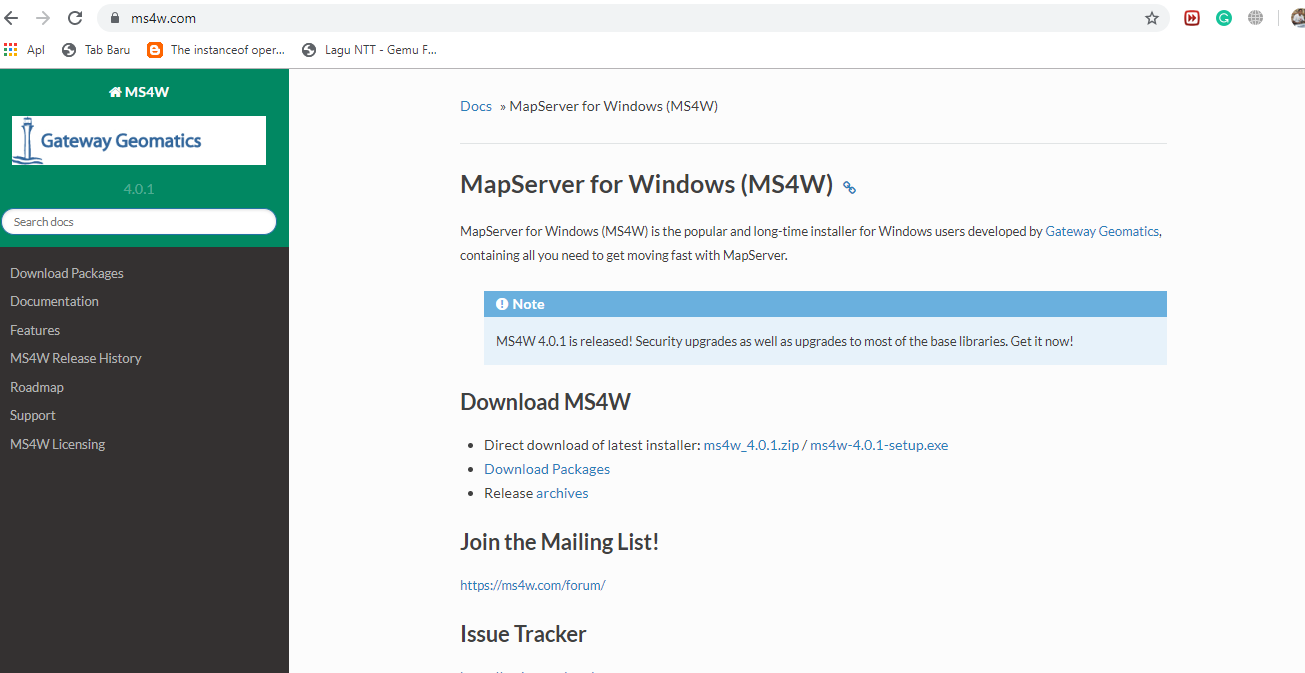
\includegraphics[width=4cm]{figures/1174096/4/g1.PNG}
		\centering
		\caption{Halaman map server untuk windows}
    \end{figure}
    \item Setelah di download, langkah selanjutnya adalah melakukan instalasi
    \hfill\break
    \begin{figure}[H]
		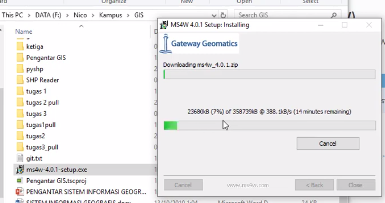
\includegraphics[width=4cm]{figures/1174096/4/g2.png}
		\centering
		\caption{proses instalasi}
    \end{figure}
    \item Instal vcredist 2017, untuk bisa menjalankan map server. untuk linknya bisa \href{https://support.microsoft.com/id-id/help/2977003/the-latest-supported-visual-c-downloads}{Klik disini}
    \hfill\break
    \begin{figure}[H]
		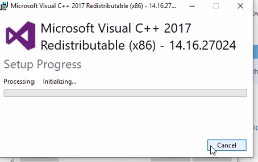
\includegraphics[width=4cm]{figures/1174096/4/g3.png}
		\centering
		\caption{proses instalasi vcredist 2017}
    \end{figure} 
\end{enumerate}
\subsection{Konfigurasi Map Server}
Jika telah selesai melakukan instalasi kita akan melakukan konfigurasi
\begin{enumerate}
  \item Buka folder ms4w
  \hfill\break
    \begin{figure}[H]
		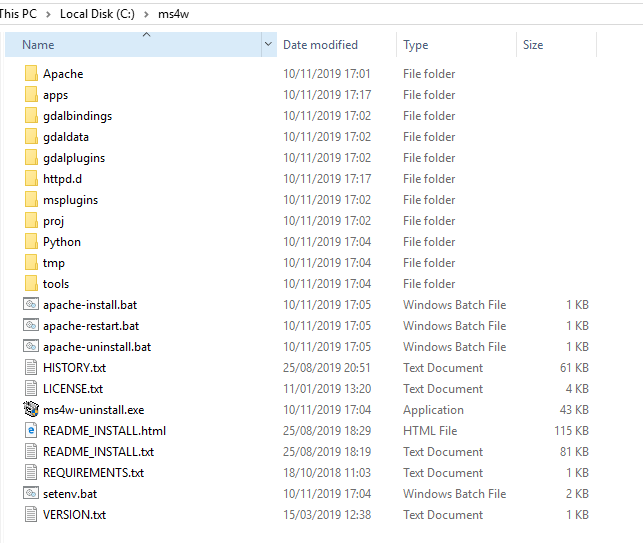
\includegraphics[width=4cm]{figures/1174096/4/g4.PNG}
		\centering
		\caption{folder ms4w pada local disk (C:)}
    \end{figure}
  \item Masuk ke folder apache dan masuk lagi ke folder conf
  \hfill\break
    \begin{figure}[H]
		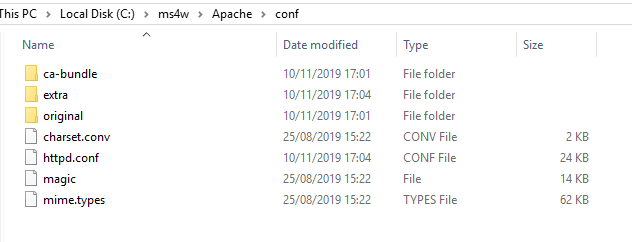
\includegraphics[width=4cm]{figures/1174096/4/g5.PNG}
		\centering
		\caption{tampilan pada folder conf}
    \end{figure}
  \item Buka file httpd.conf dan ubah listen port nya. Karena dikomputer saya port 80 digunakan untuk webserver, port ini juga bisa d setting saat proses instalasi sebelumnya.
  \hfill\break
    \begin{figure}[H]
		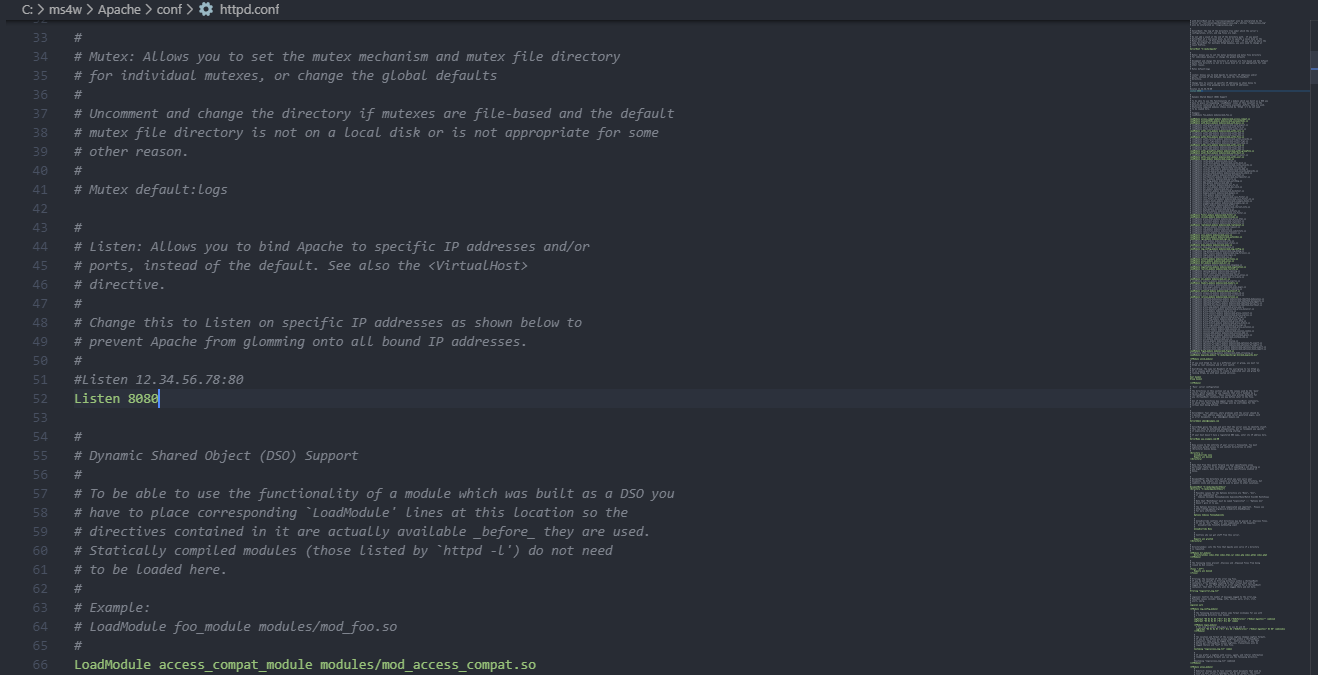
\includegraphics[width=4cm]{figures/1174096/4/g6.PNG}
		\centering
		\caption{Listen port}
    \end{figure}
  \item Kemudian kita jalankan servisnya, dengan menggunakan tombol windows + r dan ketikan services.msc
  \hfill\break
    \begin{figure}[H]
		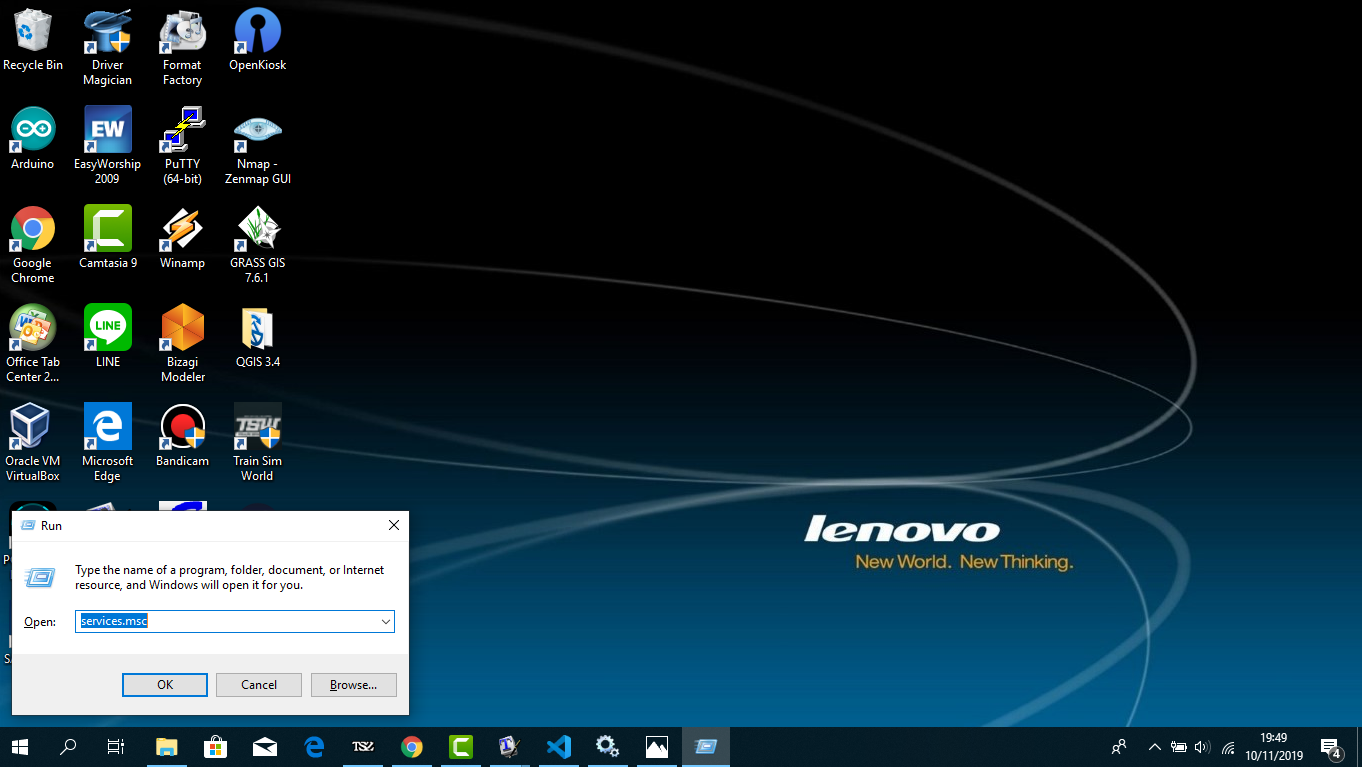
\includegraphics[width=4cm]{figures/1174096/4/g7.PNG}
		\centering
		\caption{Mengakses Halaman Service}
    \end{figure}
  \item Cari servis untuk Apache MS4W Web Server, lalu klik 2x
  \hfill\break
    \begin{figure}[H]
    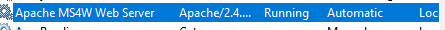
\includegraphics[width=4cm]{figures/1174096/4/g8.PNG}
    \centering
    \caption{apache}
    \end{figure}
  \item ari servis untuk Apache MS4W Web Server, lalu klik 2x
  \hfill\break
    \begin{figure}[H]
    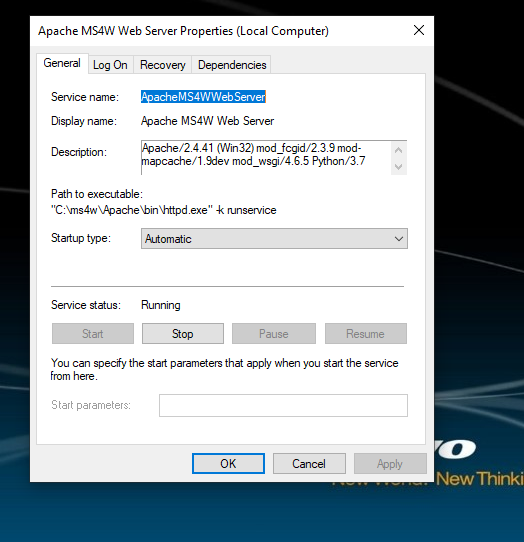
\includegraphics[width=4cm]{figures/1174096/4/g9.PNG}
    \centering
    \caption{settingan apache}
    \end{figure}
\end{enumerate}
\subsection{Pengujian}
\begin{enumerate}
  \item Masuk Ke folder httpd.d yang ada di folder ms4w kemudian buat file yang bernama httpd mywfs conf
  \hfill\break
    \begin{figure}[H]
    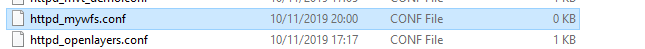
\includegraphics[width=4cm]{figures/1174096/4/g10.PNG}
    \centering
    \caption{file yang baru dibuat}
    \end{figure}
  \item Buka file httpd mywfs conf yang baru dibuat dan ubah isinya. Buka Folder apps yang ada di folder ms4w. Buat sebuah folder baru disana dengan nama mywfs,karena sebelumnya menyeting di httpd mywfs conf nya seperti itu
  \hfill\break
    \begin{figure}[H]
		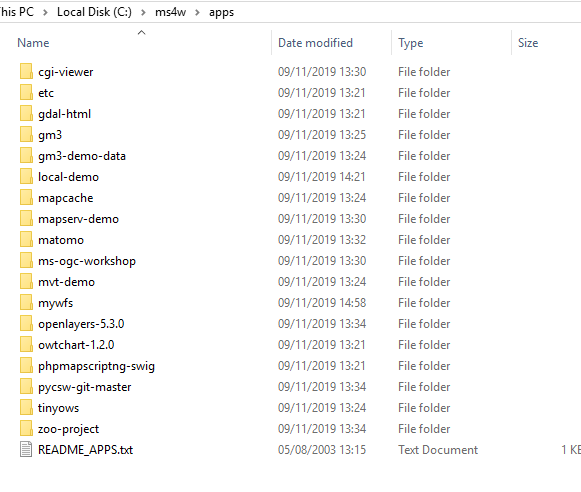
\includegraphics[width=4cm]{figures/1174096/4/g11.PNG}
		\centering
		\caption{Membuat folder baru}
    \end{figure}
  \item Modifikasi isinya menjadi sebagai berikut
  \hfill\break
    \begin{figure}[H]
		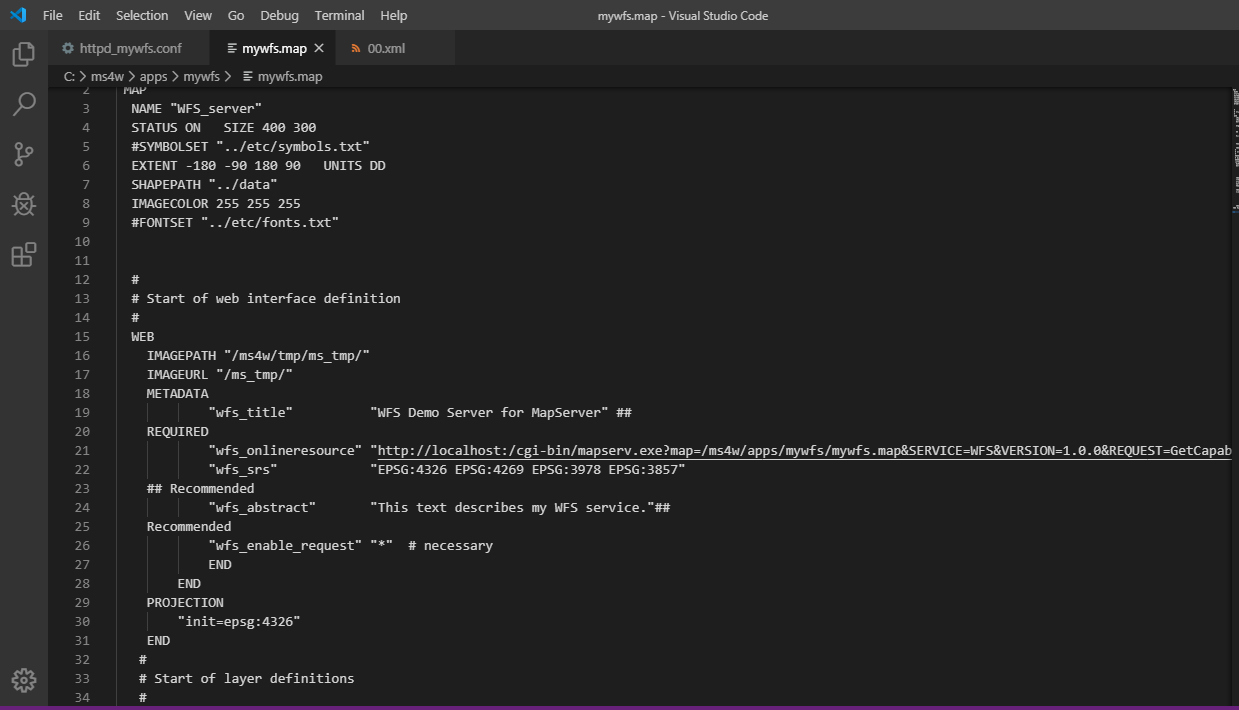
\includegraphics[width=4cm]{figures/1174096/4/g12.PNG}
		\centering
		\caption{Isi file mywfs.map 1}
    \end{figure}
    \hfill\break
    \begin{figure}[H]
		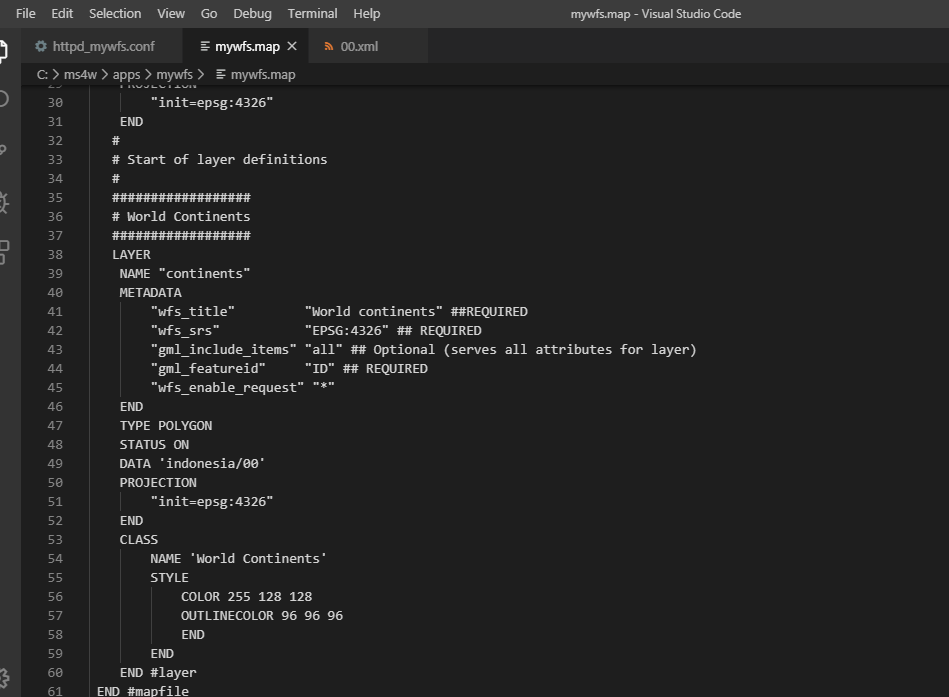
\includegraphics[width=4cm]{figures/1174096/4/g13.PNG}
		\centering
		\caption{Isi file mywfs.map 2}
    \end{figure}
  \item Kemudian Buka Browser dan \href{http://localhost:8080/cgi-bin/mapserv.exe?map=/ms4w/apps/mywfs/mywfs.map&SERVICE=WFS&VERSION=1.0.0&REQUEST=GetCapabilities}{Klik Ini}, Karena kalo diketik manual kepanjangan
  \item Nanti akan muncul tampilan XML
  \hfill\break
    \begin{figure}[H]
		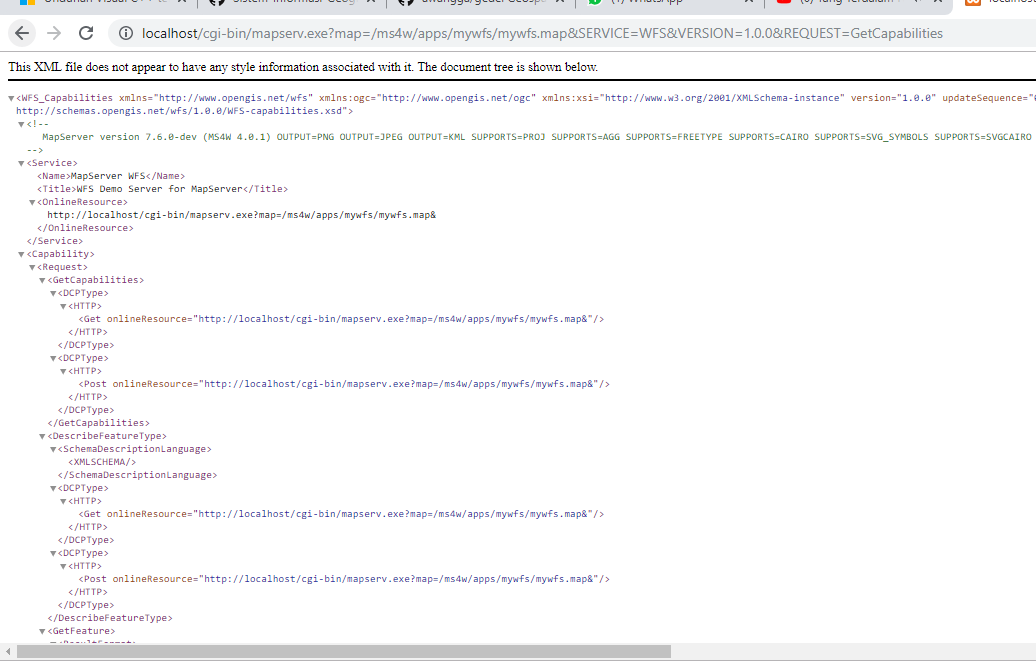
\includegraphics[width=4cm]{figures/1174096/4/g14.PNG}
		\centering
		\caption{Tampilan Web}
    \end{figure}
  \item Kemudian Copy dan Buat file baru dengan nama sesuaikan dengan .shp nya dan extensinya .xml
  \item Simpan didalam folder bersama dengan shp filenya
  \hfill\break
  \begin{figure}[H]
  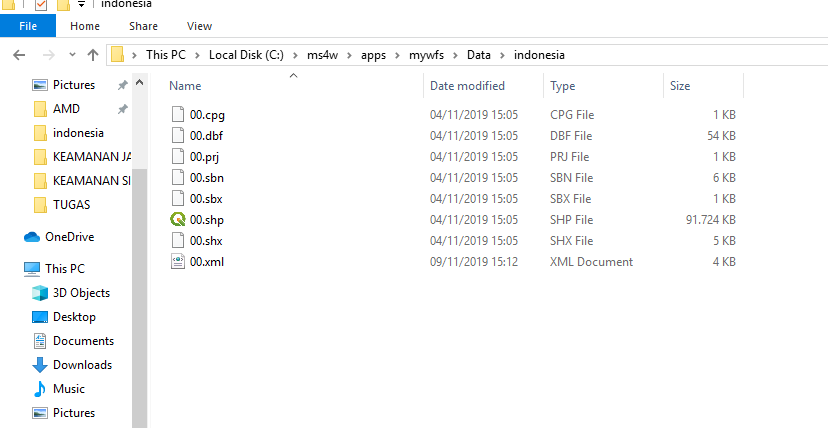
\includegraphics[width=4cm]{figures/1174096/4/g15.PNG}
  \centering
  \caption{File shp dengan XML}
  \end{figure}
  \item Dan sekarang buka file .shp nya, dan lihat hasil nya
  \hfill\break
  \begin{figure}[H]
  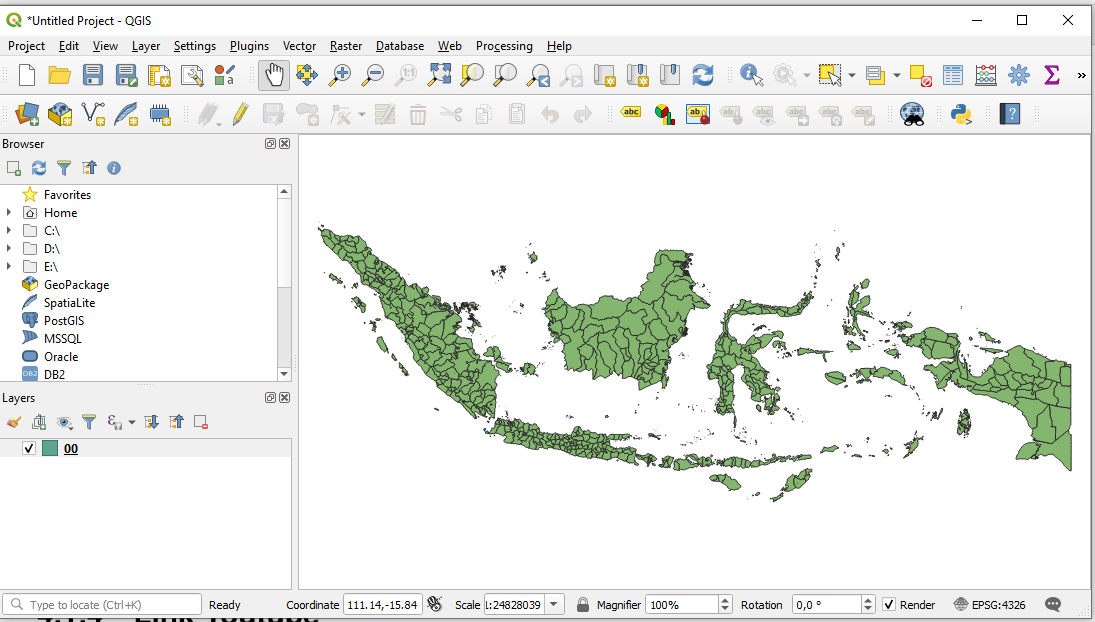
\includegraphics[width=4cm]{figures/1174096/4/g16.PNG}
  \centering
  \caption{Hasil}
  \end{figure}
\end{enumerate}
\subsection{Link Youtube}
\href{https://youtu.be/hgoMt1xKjMo}{Cek Youtube kita ya}